% The document class supplies options to control rendering of some standard
% features in the result.  The goal is for uniform style, so some attention 
% to detail is *vital* with all fields.  Each field (i.e., text inside the
% curly braces below, so the MEng text inside {MEng} for instance) should 
% take into account the following:
%
% - author name       should be formatted as "FirstName LastName"
%   (not "Initial LastName" for example),
% - supervisor name   should be formatted as "Title FirstName LastName"
%   (where Title is "Dr." or "Prof." for example),
% - degree programme  should be "BSc", "MEng", "MSci", "MSc" or "PhD",
% - dissertation title should be correctly capitalised (plus you can have
%   an optional sub-title if appropriate, or leave this field blank),
% - dissertation type should be formatted as one of the following:
%   * for the MEng degree programme either "enterprise" or "research" to
%     reflect the stream,
%   * for the MSc  degree programme "$X/Y/Z$" for a project deemed to be
%     X%, Y% and Z% of type I, II and III.
% - year              should be formatted as a 4-digit year of submission
%   (so 2014 rather than the accademic year, say 2013/14 say).
%
% Note there is a *strict* requirement for the poster to be in portrait 
% format so that we display them on the poster boards available.

\documentclass[]{templates/poster}

\usepackage{graphicx}

\DeclareGraphicsExtensions{.pdf}

\postertitle{Quantum simulation of partially distinguishable boson sampling}
\posterauthors{Alexandra E. Moylett\textsuperscript{1,2,3,*}, and Peter S. Turner\textsuperscript{1}}
\posteremail{\textsuperscript{*}alex.moylett@bristol.ac.uk}
\posteraffils{\textsuperscript{1}Quantum Engineering Technology Labs, H. H. Wills Physics Laboratory and Department of Electrical \& Electronic Engineering, University of Bristol, BS8 1FD, United Kingdom\\\textsuperscript{2}Quantum Engineering Centre for Doctoral Training, H. H. Wills Physics Laboratory and Department of Electrical \& Electronic Engineering, University of Bristol, BS8 1FD, United Kingdom\\\textsuperscript{3}Heilbronn Institute for Mathematical Research, University of Bristol, BS8 1SN, United Kingdom}

\begin{document}

% -----------------------------------------------------------------------------

\begin{frame}{} 

\begin{columns}[t]
  \begin{column}{0.422\linewidth}
  \begin{block}{\Large Main Results}
  \begin{itemize}
  \item We provide an explicit polynomial time quantum circuit for Boson Sampling with photons of arbitrary distinguishability.
  
  \item This is through reducing Boson Sampling to the problem of sampling from irreducible representations of the Unitary group [RSdG99].
  
  \item This is solvable through known circuits for the Schur transform [BCH07].
  \end{itemize}
  \end{block}

  \begin{block}{\Large 1. Boson Sampling}
  \begin{itemize}
  \item Sampling from $n$ photons on an $m$-mode interferometer.
  \begin{center}
  \begin{figure}
  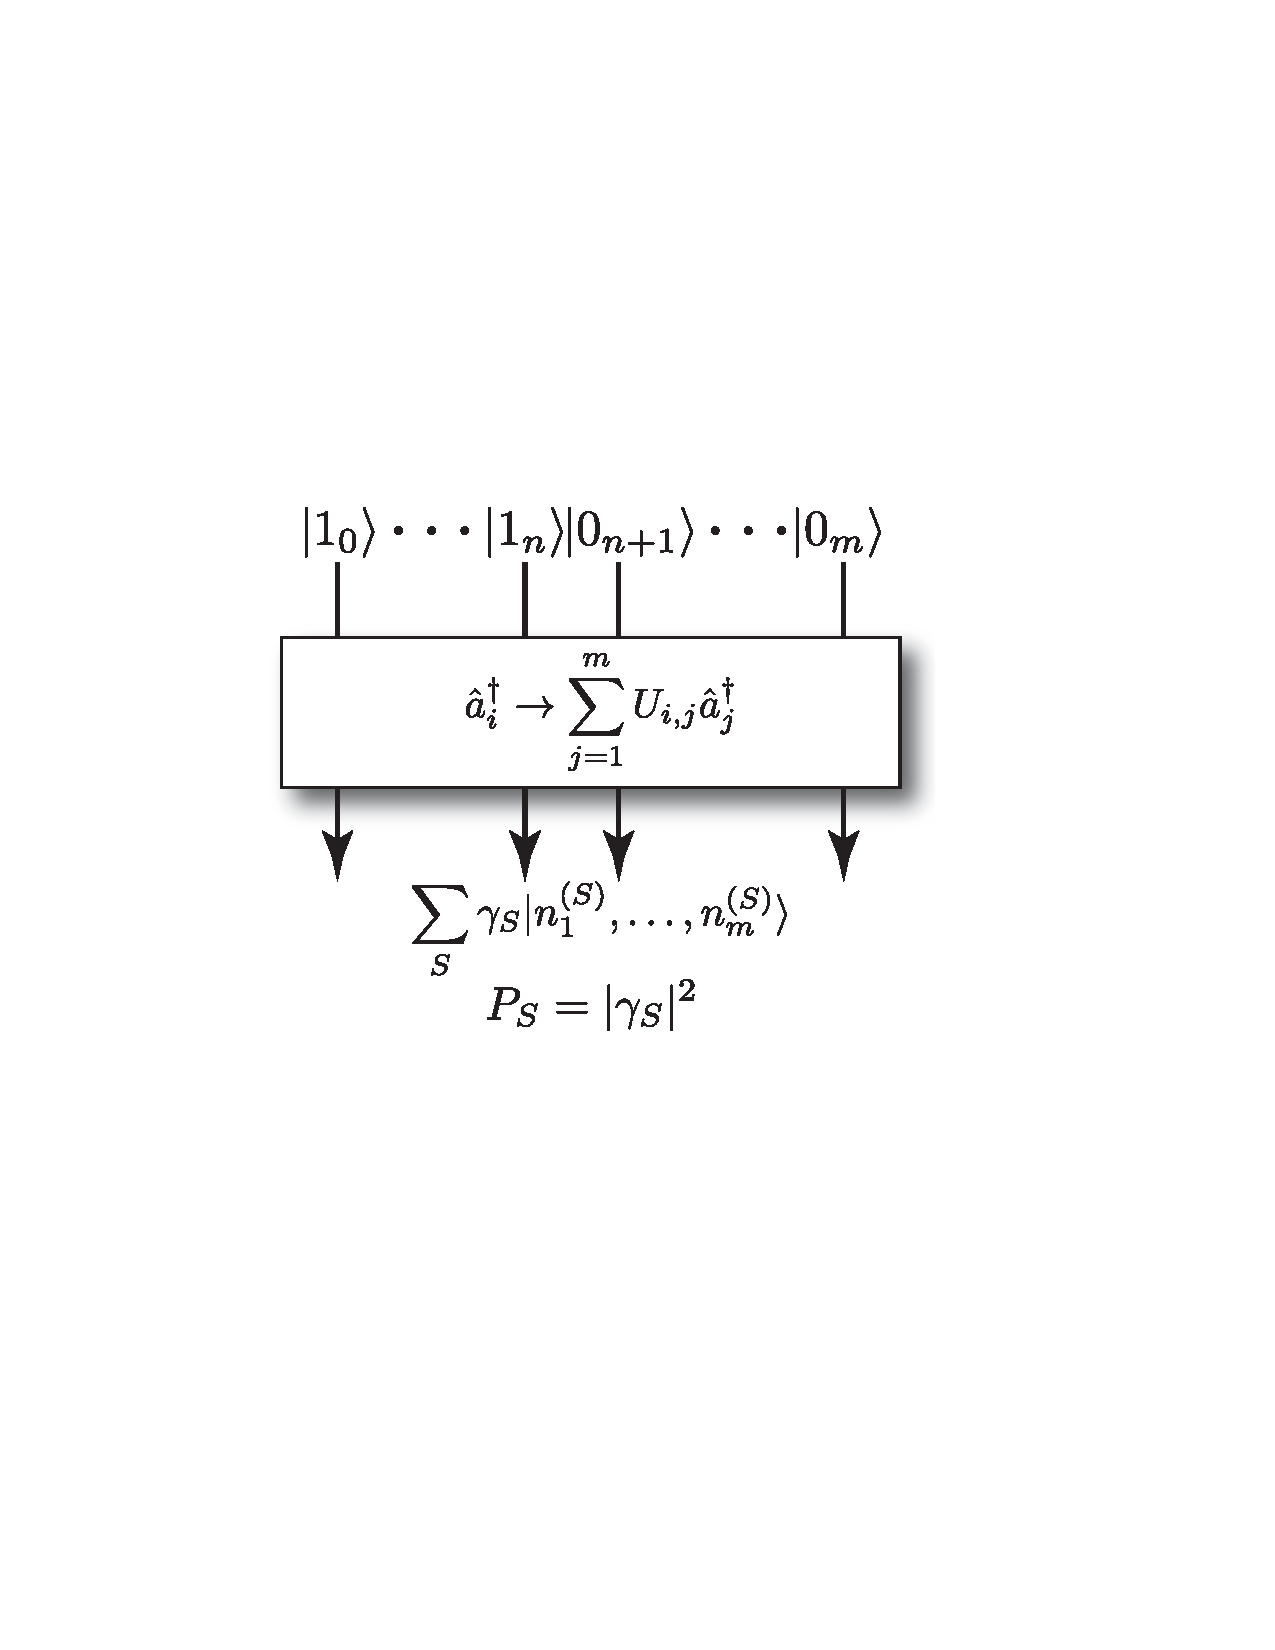
\includegraphics[width=0.4\linewidth]{model}
  \caption{\label{fig:bs} Boson Sampling model of quantum computation. Reproduced from [GMO+15]}
  \end{figure}
  \end{center}
  \item Efficient classical simulation would imply collapse of the polynomial hierarchy [AA11].
  \item Though practical algorithms for up to 50 photons exist [NSC+17].
  \end{itemize}
  \end{block}

  \begin{block}{\Large 2. Unitary group representations}
  \begin{itemize}
  \item The Hilbert space $(\mathbb{C}^{m})^{\otimes n}$ carries irreps of $\textrm{U}(m)$ and $\textrm{S}_n$.
  \item An efficient quantum circuit, denoted $W$, allows up to map between this space and the irreps [BCH08].
  
  $$W|\Psi\rangle = \sum_\lambda\sum_{q_{\lambda},p_{\lambda}}C^\lambda_{q_\lambda,p_\lambda}|\lambda\rangle|q_{\lambda}\rangle|p_\lambda\rangle$$
  
  \item There is also an efficient mapping from occupation numbers to the symmetric $\lambda=(n)$ irrep of $\textrm{U}(m)$ [RSdG99].
  \item The fully symmetric irrep of $\textrm{S}_n$ is one state, denoted $|p_{(n)=1}\rangle$.
  \end{itemize}
  \end{block}

  \begin{block}{\Large 3. Quantum circuit for Boson Sampling}
  \begin{itemize}
  \item Circuit works by creating a single particle representation of our occupation numbers through the methods in part 2.
  \item Our interferometer $U$ can then be implemented by applying $U$ to each qudit.
  \begin{center}
  \begin{figure}
  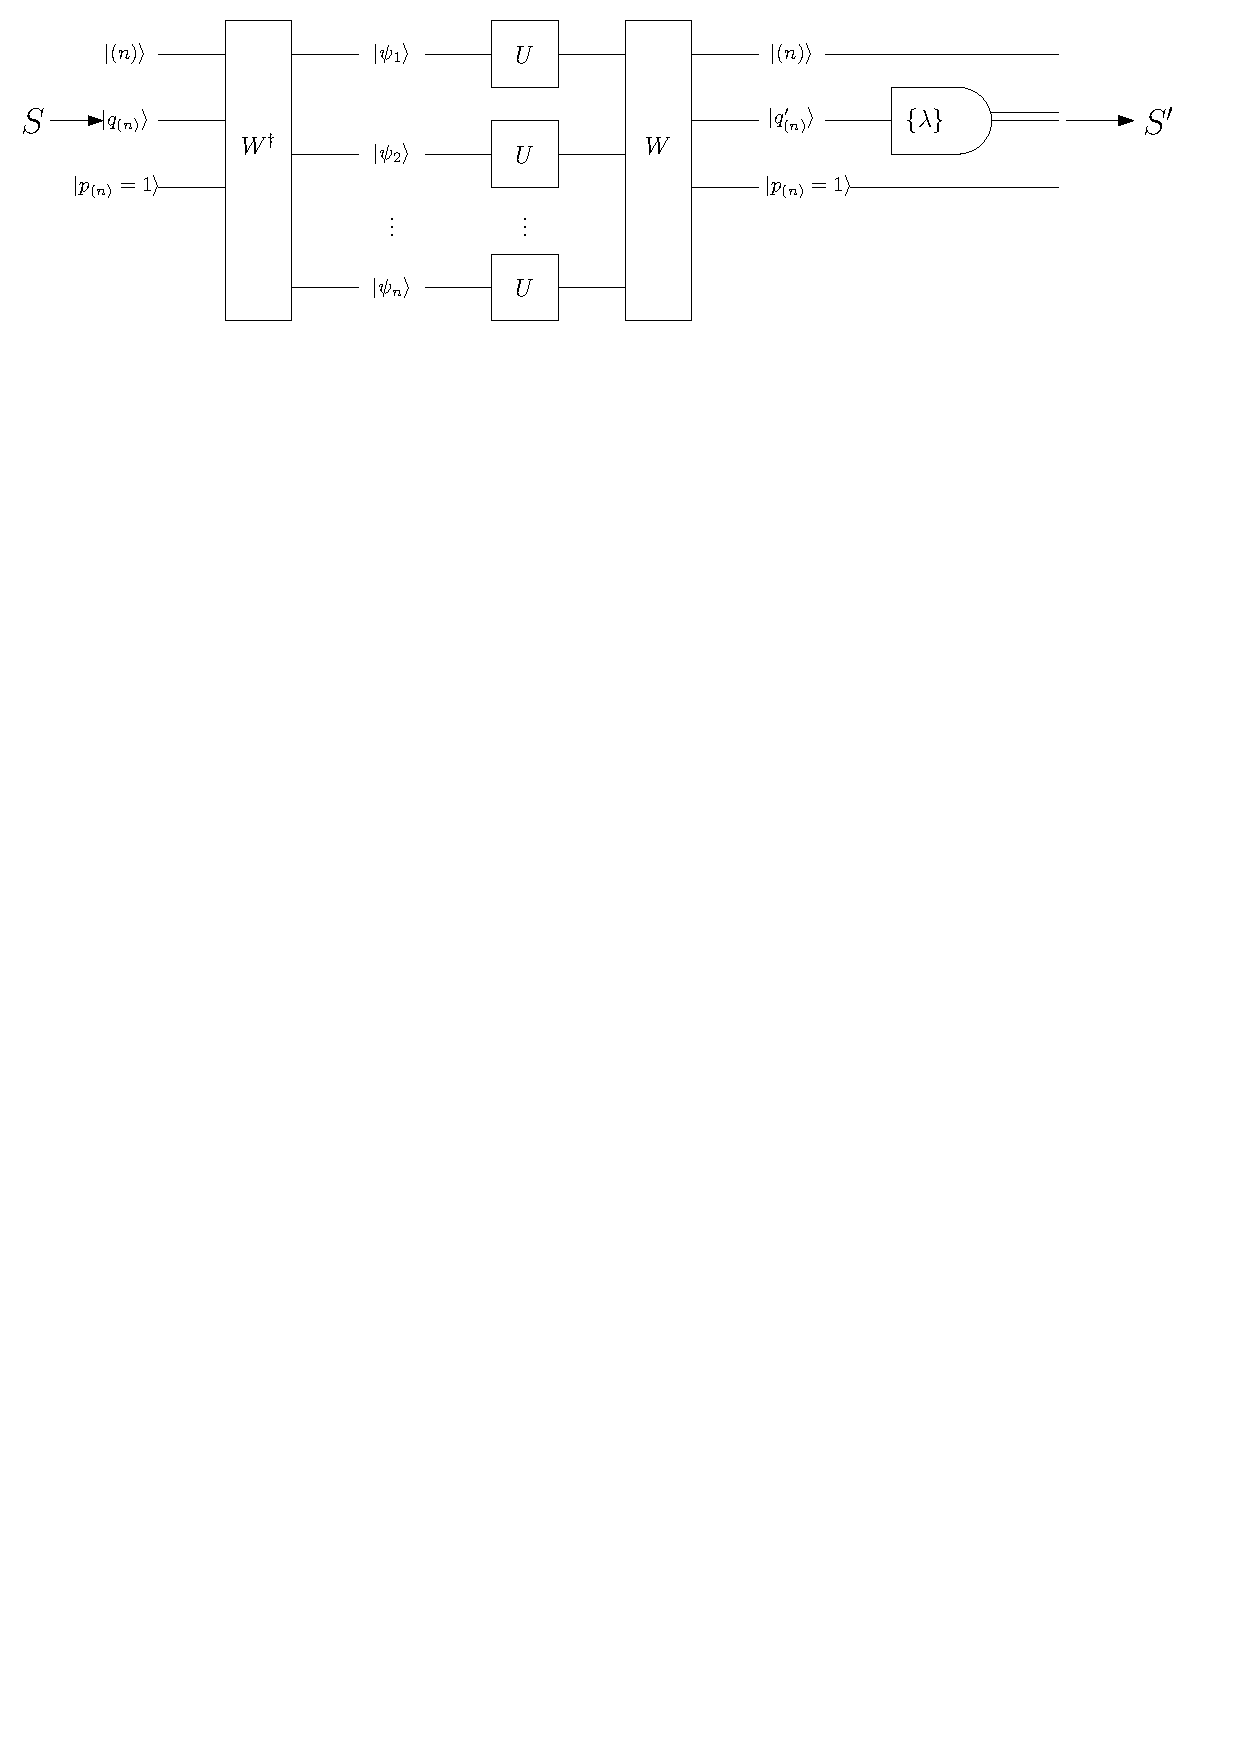
\includegraphics[width=\linewidth]{noiseless_circuit_irrep}
  \caption{\label{fig:noiseless-circuit} Circuit for Boson Sampling with indistinguishable photons. This circuit has accuracy $\delta + \epsilon$ due to approximating $U^{\otimes n}$ and $W$, and runs in polynomial time in terms of $n, m, \log\delta^{-1}$ and $\log\epsilon^{-1}$.}
  \end{figure}
  \end{center}
  \item We can also see the same distribution if we remove the second $W$ circuit and just measure each qubit in the computational basis.
  \end{itemize}
  \end{block}
  \end{column}

  \begin{column}{0.422\linewidth}
  
  \begin{block}{4. Boson Sampling with partially distinguishable photons}
  \begin{itemize}
  \item For distinguishability, we introduce a second mode.
  \item Occupation numbers map to the fully symmetric irrep of $\textrm{U}(m \times n)$.
  \item Unitary-Unitary duality decomposes this into irreps of $\textrm{U}(m)\otimes \textrm{U}(n)$ [RCR12].
  \begin{center}
  \begin{figure}
  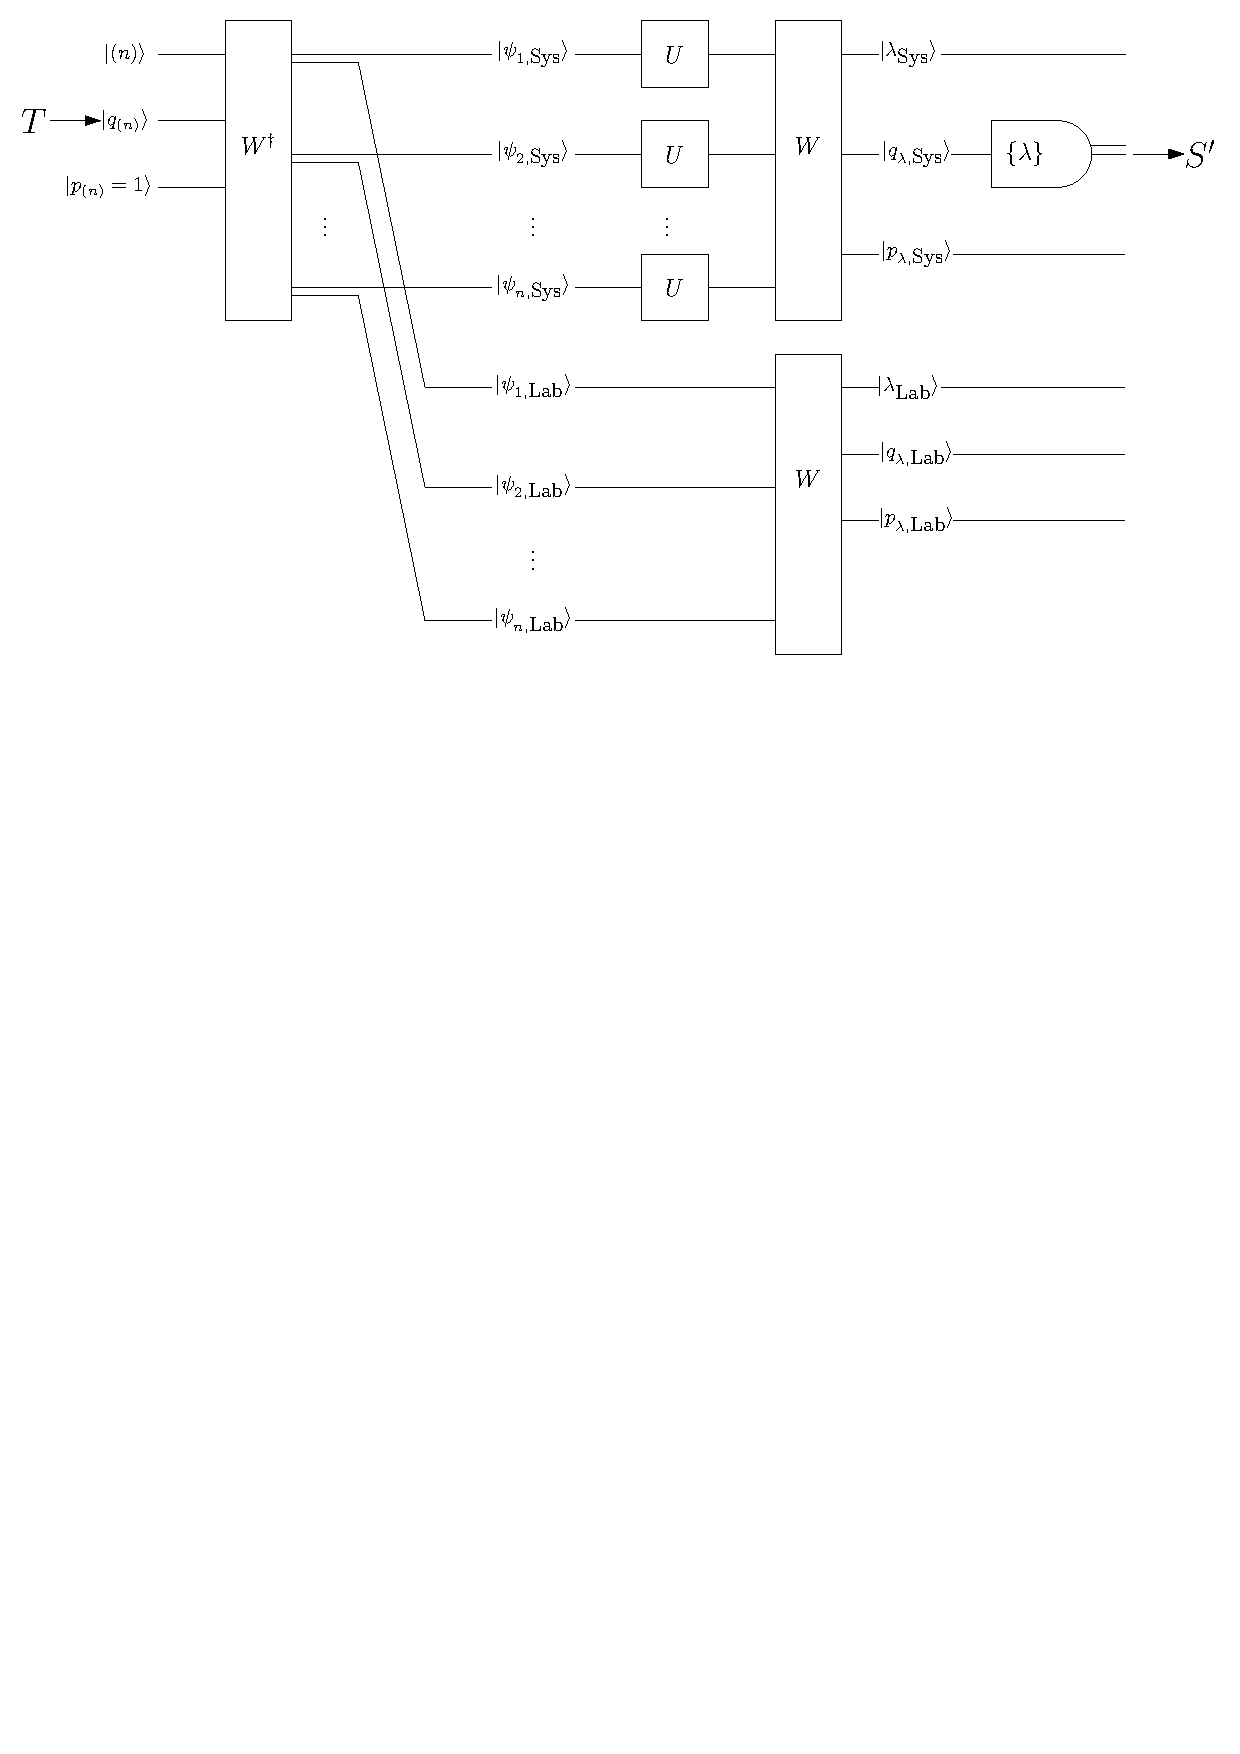
\includegraphics[width=0.75\linewidth]{noisy_circuit_rep2}
  \caption{\label{fig:noisy-circuit} Circuit for Boson Sampling with photons of arbitrary distinguishability.}
  \end{figure}
  \end{center}
  \end{itemize}
  \end{block}
  
  \begin{block}{\Large 5. Boson Sampling with loss}
  \begin{itemize}
  \item Distribution known for $n+k$ photons with $k$ lost [AB16].
  \item This can be modelled by tracing out $k$ qudits.
  \begin{center}
  \begin{figure}
  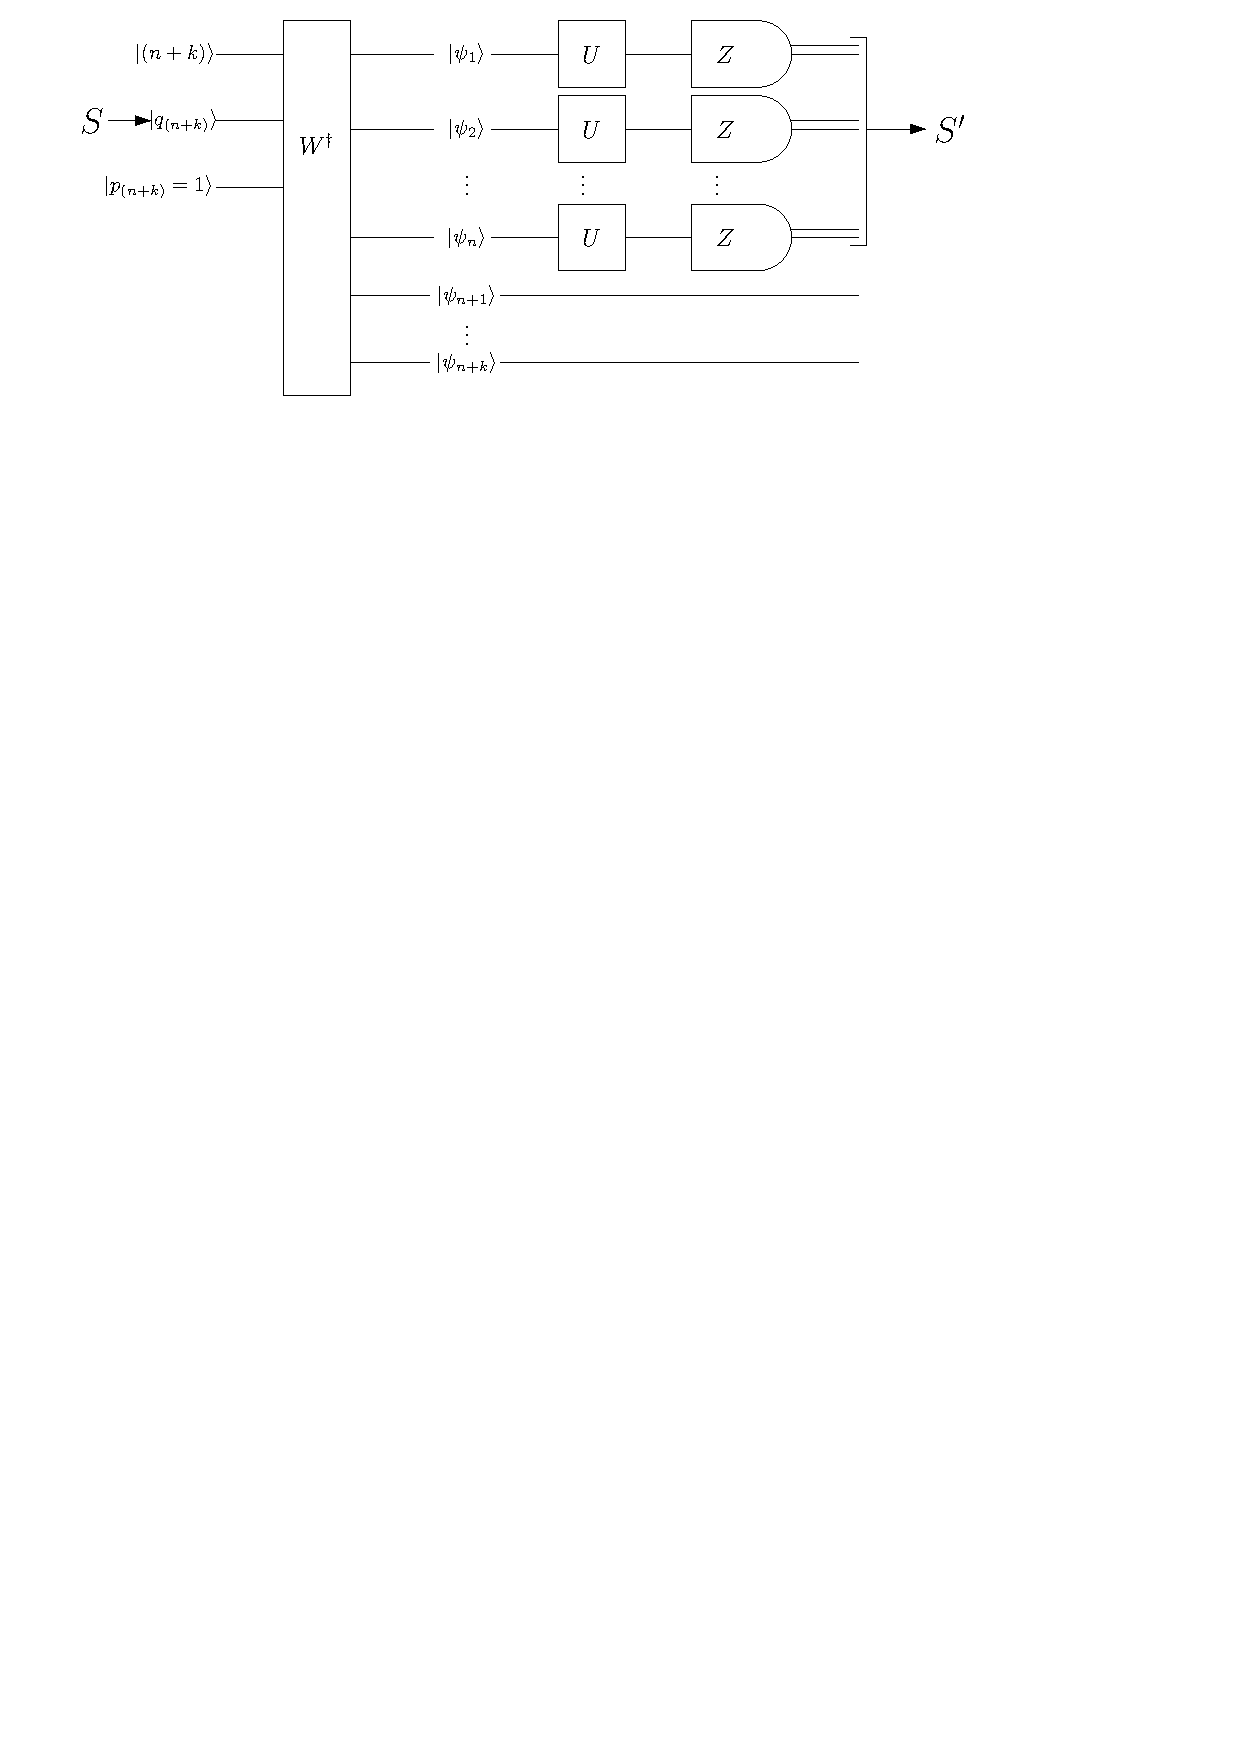
\includegraphics[width=0.75\linewidth]{lost_circuit}
  \caption{\label{fig:lost-circuit} Circuit for Boson Sampling when $k$ photons are lost.}
  \end{figure}
  \end{center}
  \end{itemize}
  
  \end{block}
  
  \begin{block}{\Large 6. Other results and future work}
  \begin{itemize}
  \item Postselecting on $|\lambda_{\textrm{Sys}}\rangle = |(n)\rangle$ allows us to perform indistinguishable Boson Sampling.
  \item Even small amounts of indistinguishability might be able to guarantee an entangled qudit state.
  \end{itemize}
  \textbf{Questions}
  \begin{itemize}
  \item Can we learn how distinguishability affects complexity?
  \item Are there any applications which irrep sampling can be used for?
  \item What do more realistic distinguishability models look like?
  \item Can we model lossy components?
  \end{itemize}
  \end{block}

  \begin{block}{\Large References}
  
  \noindent [AA11] S. Aaronson and A. Arkhipov, Proc. STOC'11, 333-342 (2011)
  
  \noindent [AB16] S. Aaronson and D. J. Brod, Phys. Rev. A \textbf{93}, 012335 (2016)

  
  \noindent [BCH07] D. Bacon, I. L. Chuang and A. W. Harrow, Proc. SODA'07, 1235--1244 (2007)
  
  \noindent [GMO+15] B. T. Gard et al., From Atomic to Mesoscale: The Role of Quantum Coherence in Systems of Various Complexities, Chapter 8 (2015)
  
  \noindent [NSC+17] A. Neville et al., Nat. Phys. \textbf{13}, 1153–1157 (2017)
  
  \noindent [RCR12] D. J. Rowe, M. J. Carvalho and J. Repka, Rev. Mod. Phys. \textbf{84}, 711-757 (2012)
   
  \noindent [RSdG99] D. J. Rowe, B. C. Sanders and H. de Guise, J. Math. Phys., \textbf{40} 7, 3604-3615 (1999)
  \end{block}
  \end{column}
\end{columns}

\end{frame}

% -----------------------------------------------------------------------------

\end{document}



